\documentclass{llncs}
\usepackage{times}
\usepackage{calc}
\usepackage{graphicx}
\usepackage{multirow}
\usepackage{colortbl}
\usepackage{rotating}
\usepackage{array}
\usepackage[usenames,dvipsnames]{xcolor}
\usepackage{ifthen}
\usepackage{amssymb}
\newboolean{showcomments}
\setboolean{showcomments}{true} % toggle to show or hide comments
\usepackage{cite}
\usepackage{listings}
\lstset{ %
  backgroundcolor=\color{white},   % choose the background color; you must add \usepackage{color} or \usepackage{xcolor}
  basicstyle=\scriptsize,        % the size of the fonts that are used for the code
  breakatwhitespace=false,         % sets if automatic breaks should only happen at whitespace
  breaklines=true,                 % sets automatic line breaking
  captionpos=b,                    % sets the caption-position to bottom
  commentstyle=\color{mygreen},    % comment style
  deletekeywords={...},            % if you want to delete keywords from the given language
  escapeinside={\%*}{*)},          % if you want to add LaTeX within your code
  extendedchars=true,              % lets you use non-ASCII characters; for 8-bits encodings only, does not work with UTF-8
  frame=single,                    % adds a frame around the code
  keepspaces=true,                 % keeps spaces in text, useful for keeping indentation of code (possibly needs columns=flexible)
  keywordstyle=\color{blue},       % keyword style
  language=xml,                 % the language of the code
  morekeywords={*,...},            % if you want to add more keywords to the set
  numbers=none,                    % where to put the line-numbers; possible values are (none, left, right)
  numbersep=5pt,                   % how far the line-numbers are from the code
  %numberstyle=\tiny\color{mygray}, % the style that is used for the line-numbers
  rulecolor=\color{black},         % if not set, the frame-color may be changed on line-breaks within not-black text (e.g. comments (green here))
  showspaces=false,                % show spaces everywhere adding particular underscores; it overrides 'showstringspaces'
  showstringspaces=false,          % underline spaces within strings only
  showtabs=false,                  % show tabs within strings adding particular underscores
  stepnumber=2,                    % the step between two line-numbers. If it's 1, each line will be numbered
  %stringstyle=\color{mymauve},     % string literal style
  tabsize=2,                       % sets default tabsize to 2 spaces
  title=\lstname                   % show the filename of files included with \lstinputlisting; also try caption instead of title
}

\ifthenelse{\boolean{showcomments}}
  {\newcommand{\nb}[2]{
    \fcolorbox{gray}{yellow}{\bfseries\sffamily\scriptsize#1}
    {\sf\small$\blacktriangleright$\textit{#2}$\blacktriangleleft$}
   }
   \newcommand{\version}{\emph{\scriptsize$-$working$-$}}
  }
  {\newcommand{\nb}[2]{}
   \newcommand{\version}{}
  }

\ifthenelse{\boolean{showcomments}}
  {\newcommand{\rev}[1]{\textcolor{red}{#1}}}
  {\newcommand{\rev}[1]{#1}}

\renewcommand{\labelitemi}{$\bullet$}
\setlength{\textfloatsep}{3mm}
\setlength\intextsep{3mm}

\usepackage[hyphens]{url}

\begin{document}
\title{CMS-CL : A DSL to simplify the configuration of Content Management Systems}
\author{Matthieu Allon, Jordi Cabot}
\institute{AtlanMod team (Inria, Mines Nantes, LINA), Nantes, France\\ \email{\{matthieu.allon,jordi.cabot\}@inria.fr}}
\maketitle

\begin{abstract}
%One short sentence describing state of the art
The websites development was simplified over time, notably via
the Web standardization, but also through the use of CMS \footnote{Content Management System}.\\
%One / two short sentences desc. drawbacks
However, the use of the various available tools still requires technical knowledge, that web designers have (concerning CMS itself, web standards, or databases), unlike many end users (which can be an obstacle to the web site creation).\\
%One short sentence desc. conceptual solution(s) presented in the paper
In this paper, we propose a simplification of the website creation for end users and, for web designers, an improvement of the configuration of one or several sites.\\
%One - Three sentences desc. advantages of choosen conceptual solutions
Allowing end users to create their websites will enable them to implement their ideas directly, without being slowed by technical points, but also to reduce the gap between concepts and practice. Simplification for web designers will let them to configure and manage easier and quicker their  website(s).\\
% One - three sentences desc. implementation of choosen conceptual solutions
So we create a DSL\footnote{Domain Specific Language}~\cite{dsl} and its metamodel~\cite{metaExplanation} to represent the general structure of a website configured via the WordPress CMS (which is the most used one currently~\cite{cmsRepartition}). By using the DSL metamodel and the mind mapping (via a software~\cite{freeplane} extension), we enabled end users to create their site simpler.\\
For web designers, we integrate the DSL in an IDE\footnote{Integrated Development Environment}, via an Eclipse product\cite{eclipseProduct} and the use of the XText Eclipse plugin~\cite{xtext}, to have a configuration file for one or several websites (and therefore to configure them remotely).\\
\keywords{Website developement, CMS, DSL, Mind mapping}
\end{abstract}
\section{Introduction}
Nowadays, many tools are available on the market to simplify and speed-up the development of websites. Such tools can provide support for static (e.g. the DreamWeaver, WebExpert, ... editors) or dynamic (e.g. the Drupal, Joomla, ... CMS) websites. The most widely used tools are CMS (Content Management System - about 60\% of the current websites use a CMS \cite{cmsRepartition}): it brings clear adavantages\cite{cmsAdvDraw}, with respect to other methods and tools.

%CMS drawbacks
Unfortunately, CMS have drawbacks for end-users: the technical knowledge (e.g. plugins, theme, ...) to use it, the lack of default functionalities (e.g. for Search Engine Optimization, ECommerce, Social Networks ...), the concepts scattering and the lack of participation of end-users in website creation.

Hence, we have created a DSL\cite{dslDefine} (named 'CMS-CL': CMS Configuration Language) which has all concepts present in WordPress, with some default functionalites (e.g. Search Engine Optimization, anti-spam, multi-language, ...). With this DSL, users focus only on the conceptual side (e.g. relations between a post and a page, ...).

We have decided to use a specific representation with our DSL: the mind-mapping. It is a way to represent concepts: each one is symbolized as a node (the root/central node being the main concept), and the various relations between these concepts are represented through edges. The mind-mapping allows to easily manipulate the different DSL concepts, to have all of it in one view and to enable end-users to be less partisan of a wait-and-see by participating more in the website creation, and therefore exchanging more with web designers and other members of a website project.

We have implemented a prototype using our DSL with a mind-mapping based notation. Then, we made an experiment of this tool with end users, to validate its interest.

This paper presents the design and how to use the DSL through the following sections : the approach overwiew (Section \ref{approachOverview}), a presentation of our DSL and its syntax (Section \ref{CMS-CL}), a presentation of the implementation (Section \ref{techUse}), the CMS-CL prototype validation (Section \ref{validation}), CMS-CL and the web designers (Section \ref{webDesigners}), the related work (Section \ref{relatedWorks}) and a conclusion about this approach.
\section{Approach overview} \label{approachOverview}

	\begin{figure}[!h]
		\centering
		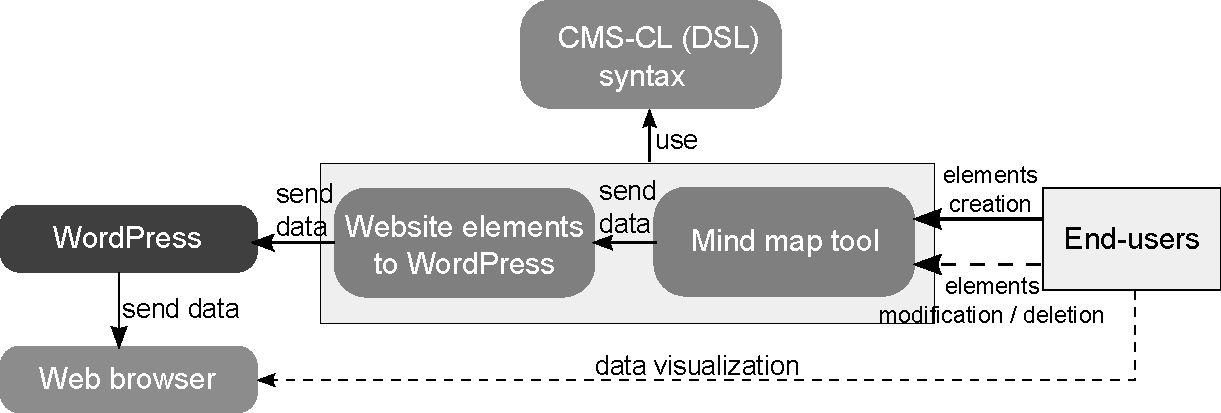
\includegraphics[width=\textwidth]{../resources/pdf/endUsersSimplifiedPresentation.pdf}
		\caption{CMS-CL and mind mapping use}
		\label{CMS-CLMindMappingUse}
	\end{figure}

	As it is presented in Fig.\ref{CMS-CLMindMappingUse}, the use of our defined DSL 	('CMS-CL') with the mind mapping is the following :	
	
	\vspace{0.15em}
	\noindent\textbf{Elements creation.} Using a GUI \footnote{Graphical User Interface}, end users are able to create some website elements.	
	
	\vspace{0.15em}
	\noindent\textbf{Mind-mapping metamodel reduction.} The mind mapping metamodel is reducted to the elements of the CMS-CL metamodel (paragraph \ref{abstractSyntax}). Then, data (elements) are injected into the WordPress platform.	
	
	\vspace{0.15em}
	\noindent\textbf{Data visualization.} After the data injection, it is possible to see the changes on the web site, via a web browser.	
	
	\vspace{0.15em}
	\noindent\textbf{Elements modification and/or deletion.}
	
	\vspace{0.15em}
	\noindent\textit{Deletion:} Users just have to put a delete icon
	(
\includegraphics[scale=0.50]{../resources/png/delete.png}) as described in the section \ref{CMS-CL}, paragraph \ref{concreteSyntax}.
	
	\vspace{0.15em}
	\noindent\textit{Modification:} Users must have to delete first the corresponding element, and recreate a new one with the 					modification. The only exception concerns the 'Website' root node, because it is mandatory : its attribute can be directly modified.	
\section{CMS-CL (CMS Configuration Language)}\label{CMS-CL}		
'CMS-CL' is a DSL. A DSL\cite{dslDefine} is a computer language for a specific domain (e.g. SQL, HTML, OCL, ...) : its syntax are designed to work in the targeted domain as good as possible. This syntax is composed of three parts : the \textit{abstract syntax} is the unvariable part (i.e. the structure of the language) without any particular representation. The \textit{semantics part} is about the meaning of the elements, and the \textit{concrete syntax} concerns the variable part, which describes the representation of the language. 
In the following sections, the CMS-CL syntaxs and semantics are detailed.		
			
			\subsection{CMS-CL Abstract Syntax and Semantics}\label{abstractSyntax} 
The DSL created for the website management contains several features allowing configuration modifications and creations by users. These elements have been represented in a metamodel~\cite{metaExplanation}: for the sake of conciseness, we do not show the entire metamodel\footnote{\scriptsize{CMS-CL complete metamodel: \url{https://raw.github.com/mallon/WordPress-MindMapping/master/Documentation/DetailedFigures/WdpDslCompleteMM.pdf}}}, but a simplified one in Fig.\ref{CMS-CLMetamodel}.
				\begin{figure}[!h]
					\centering
					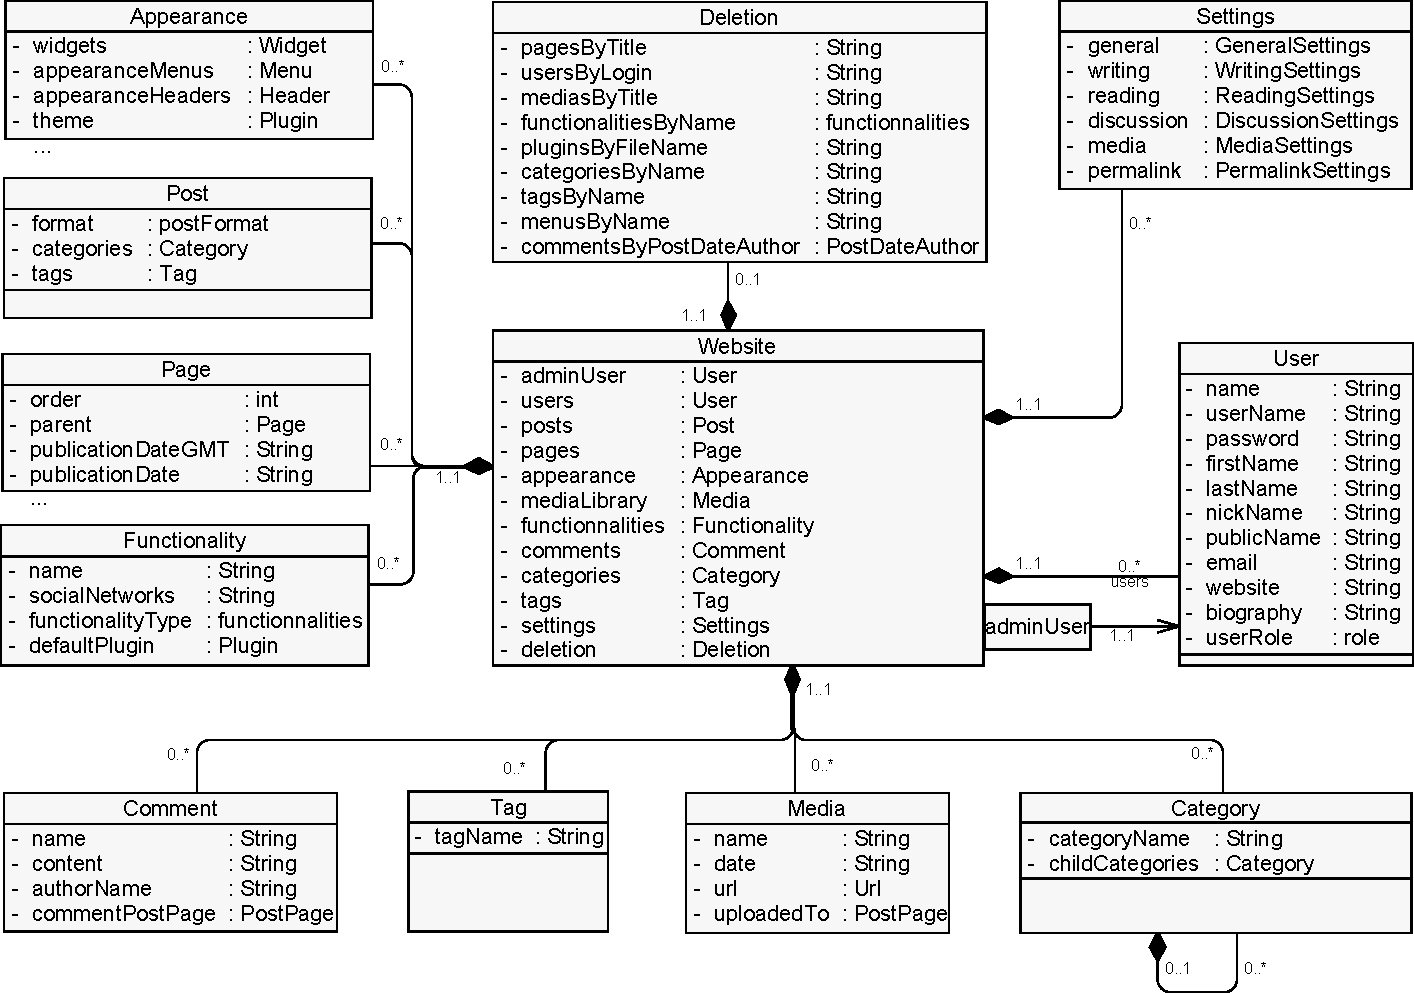
\includegraphics[width=\textwidth]{../resources/pdf/WOCMMSimplified.pdf}
					\caption{CMS-CL simplified metamodel (abstract syntax)}
					\label{CMS-CLMetamodel}
				\end{figure}	
							 								
\vspace{0.15em}
\noindent\textbf{User. \label{userElement}} With this concept, it is possible to create users with their mandatory respective roles (granting rights to the various elements of the site) : \textit{'Administrator', 'Editor', 'Author', 'Contributor' and 'Suscriber'}. It is important to notice that users modifying the website configuration  must have an administrator role, which is represented by the element \textit{'AdminUser'} (by default the users are connected with the administrator account automatically created during the WordPress server installation).
 
\vspace{0.15em}
\noindent\textbf{Appearance.}End users will be able to change the appearance of the website, using the elements of 'Appearance'. The \textit{'apperanceHeader'} and \textit{'theme'} elements will respectively change the header of the site's main page and select a new theme. Its modification will influence how other features appear (e.g. the placement of the page on the website). For the 'Theme' feature, there are six default themes, choosen accordingly to the list of the most popular ones in 2013 \cite{topTheme} : \textit{Responsive, Magazine, Business, Galleries, Artistic and SEO}. 
The item \textit{'Menus'\label{menu}} allows changing the default content of the navigation elements. It is possible to change the default  access to the pages and posts, by creating a new item \textit{'Menu'} with external links (\textit{'Links'}), pages/posts categories (\textit{'Categories'}) or pages (\textit{'Accessed pages'}). 
Furthermore, end users can add functionalities to the site (and are displayed regardless of the page/post) with the twelve default \textit{'Widgets'}.

\vspace{0.15em}
\noindent\textbf{Deletion.} This entity contains all the names of the various items that the user wish to delete.

\vspace{0.15em}
\noindent\textbf{Comment.} It represents the comments write by users on a page/post.

\vspace{0.15em}
\noindent\textbf{Category.} Each categories can be composed in sub-categories. For instance, it can exists a category 'Music' containing two sub-categories 'Group' and 'Concert'.

\vspace{0.15em}
\noindent\textbf{Media.} This feature corresponds to images and videos which can be inserted with the content.

\vspace{0.15em}
\noindent\textbf{Tag.} It allows to find various posts concerning a same subject. Navigation within a website can be easy through the use of tags in order to find a particular information : for this reason, a tag can be added to a post.

\vspace{0.15em}
\noindent\textbf{Functionality.} Users usually wish to customize their web site according to their needs. Hence, a set of default functionalities is provided: \textit{eCommerce, spam, indexing, multilanguage, seo, pictures, and social Networks}. The users may select a functionality among them , or install another one ('plugin' attribute).

\vspace{0.15em}
\noindent\textbf{Page and Post.} Users (which have the correct rights) can add posts. Pages can be also added, and for this two elements, the author correspond to the administrator account of the user (see 'User' details \ref{userElement}). 

\vspace{0.15em}
\noindent\textbf{Settings.} 
It contains the various types of configuration : \textit{General, Writing, Reading, Media} and \textit{Permalinks}. In the \textit{GeneralSettings} class, \textit{login} and \textit{administrator} password attributes are required to enable the connection (to the platform site creation) which is realized with the platform \textit{address} attribute. But the settings require more technical knowledges, therefore the end-users will not have the possibility to modify it : only the web-designers will be able to do this (section \ref{webDesigners}).
				
			\subsection{CMS-CL Concrete Syntax}\label{concreteSyntax}	
			   	In the next two paragraphs, we present the tool used to represent a mind-map and the CMS-CL concrete 
			   	syntax, which is the visual representation. A mapping between the metamodel concepts (the abstract 
			   	syntax) and this visual representation (the mind-mapping) was necessary.
			   	
			   \vspace{0.15em}
			   \noindent\textbf{Representation Tool used.}\label{representationTools}
			   			There are a lot of different softwares for mind	mapping, and FreeMind was during a long time of those who
			   			have different interesting features : popularity, soundness, interactiveness, open 
			   			source, extensibility, export facilities and scripting. A fork of FreeMind was created: Freeplane. It 								provides and improves some of the 
			   			points mentioned above: a regularly updating and an improved extension system~\cite{freeplane}.
																	
				\vspace{0.15em}
				\noindent\textbf{CMS-CL and mind-mapping.} A mind-map is a diagram used to present concepts (or other items like tasks). There is one central governing concept, which is in the center of this 							diagram, and each other concepts are related to it. Each idea is symbolized as a child node of the central node (i.e. the central concept), and the 							various relations between these concepts are represented through edges. The software presented above adds the possiblity to create attributes for a 								node : an attribute is a node property (e.g. an address for a website).
									
						\begin{figure}[!h]
							\centering
							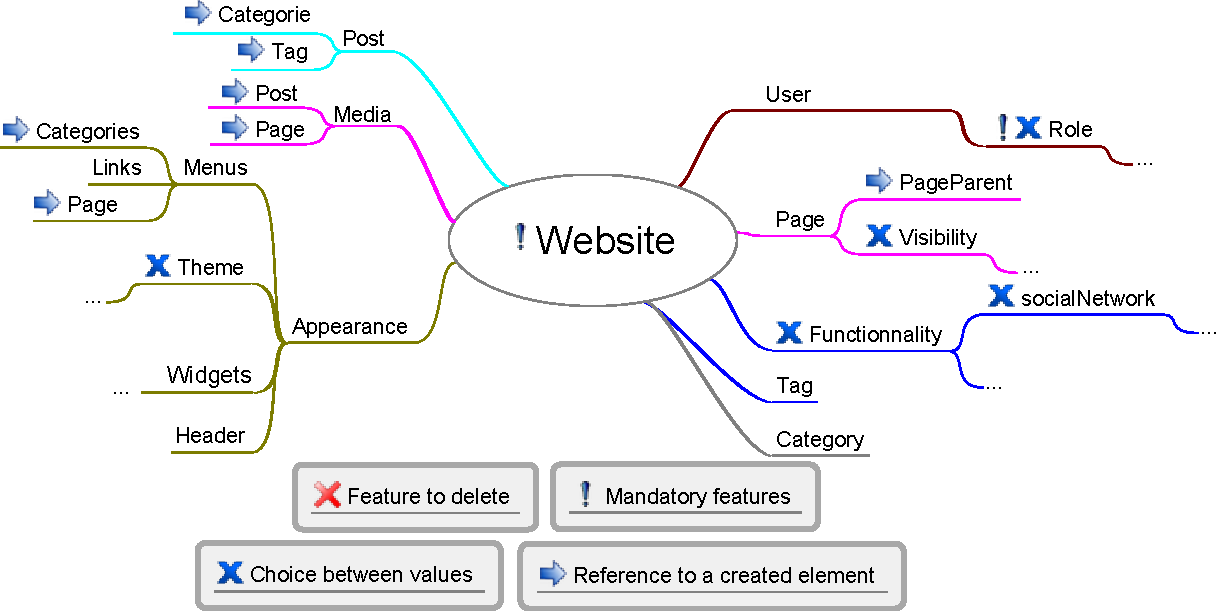
\includegraphics[width=0.85\textwidth]{../resources/pdf/CMS-CLFeatures.pdf}
							\caption{CMS-CL on top of the FreePlane metamodel (simplified representation)}
							\label{websiteDSLFeatures}
						\end{figure}
						The various concepts, their parameters and relationships are respectively represented by nodes, 
						attributes, and edges. CMS-CL has a visual representation via the mind mapping and it is on top of the Freeplane metamodel. 
						To adapt our DSL to this metamodel\footnote{\scriptsize{FreePlane metamodel: \url{https://raw.github.com/mallon/WordPress-MindMapping/master/Documentation/DetailedFigures/FreeplaneMM.pdf}}} 
						, it was necessary to make a 'CMS-CL-to-FreePlane' mapping\footnote{\scriptsize{'CMS-CL-to-FreePlane' mapping: \url{https://raw.github.com/mallon/Word-PressMindMapping/master/Documentation/DetailedFigures/CMS-CL2FreePlane.pdf}}} 
\footnote{\scriptsize{Schematique representation: \url{https://raw.github.com/mallon/Word-PressMindMapping/master/Documentation/DetailedFigures/CMS-CLFeaturesComplete.pdf}}}.
						
						\vspace{0.15em}
						\noindent\textbf{Website.} It is the root node, which represents the web site to create, with its title, tagline, 	
						login and administrator password attributes. 
						
						\vspace{0.15em}
						\noindent\textbf{Appearance.}Directly connected to the root node, it contains four child nodes : \textit{Widget}, 
							\textit{Menu}, \textit{Header} and \textit{Theme}. Each of this fourth child nodes have also child 	nodes. 
											
						\vspace{0.15em}
						\noindent\textbf{User.} Child node of the 'Website' root node. It has a child node \textit{Role}.
						
						\vspace{0.15em}
						\noindent\textbf{Page.} Child node of the 'Website' root node. Its title and content
						are defined by its first two attributes: 'title' and 'content'. His child node \textit{'PageParent'}
						represents the page to be displayed with it (in the site menu bar by default). The definition of the attribute 
						'order' within the parent node \textit{'Page'} allows you to change the order. Because a page can be public or 
						private, a second child node was added to the node \textit{'Page'} : \textit{'Visibility'}.
						
						\vspace{0.15em}
						\noindent\textbf{Post.} Child of the root node, it is an article posted by a user. It contains two child nodes
						referencing existing other nodes : \textit{Category} and \textit{Tag}.						
						
						\vspace{0.15em}
						\noindent\textbf{Tag and Category.} Child of the root node, with their attributes 'name' and 'description'.
																						
						\vspace{0.15em}
						\noindent\textbf{Functionality.} Child of the root node, it has seven child nodes. It is possible to choose only 		
						one of them. For the functionalities concerning social networks, two children nodes of the \textit{'SocialNetwork '} 
						node can be	added (\textit{'facebook'} or \textit{'twitter'}).	
						
						\vspace{0.15em}
						\noindent\textbf{Media.} Child of the root node, it has \textit{Page} and \textit{Post} nodes as child. Each of
						them has an \textit{arrow} icon, to be related to others existing \textit{Post} or \textit{Page} nodes.
									
						\vspace{0.15em}
						\noindent\textbf{Settings.} Because the targeted user for the mind-mapping is users with a low technical knowledge, 							the 'Settings' are not represented in this visual concrete syntax, but in the textual one (\ref{webDesigners}), 								concerning web-designers.						
										
						\vspace{0.15em}
						\noindent\textbf{Constraints.} There are some constraints on the FreePlane mind map, because a CMS-CL expression 
						is conform to a FreePlane model,
						but not the opposite. This conformity is determined by the CMS-CL abstract syntax, and we can see the various
						constraints on the figure \ref{websiteDSLFeatures}, with the four free nodes, used as keys. To summarize, the 									constraints are the following :
						
						\vspace{0.15em}
						\noindent\textit{Deletion:} To delete a website element, it is necessary to add the delete icon
											(
\includegraphics[scale=0.50]{../resources/png/delete.png}) on the targeted elements. More precisely, the elements which support this delete icon are those with attributes (excepted the 'Website' root node, which is mandatory), or 		with a choice concerning their child nodes (so, the nodes with a cross icon).
							
						\vspace{0.15em}
						\noindent\textit{Mandatory features:} Some elements are mandatory, as the child node \textit{Role} of \textit{User}, or the three 												attributes of the \textit{Website} root node : \textit{address, adminPassword and adminLogin}. The icon used is the 													\textit{Exclamation mark} one (
\includegraphics[scale=0.50]{../resources/png/exclamationMark.png}).
						
						\vspace{0.15em}
						\noindent\textit{Choice:} Several nodes have several child nodes, but it is possible to choose only one of them. It is the case for the 
									functionalties or the themes. The icon used is the \textit{Cross} one (
\includegraphics[scale=0.50]{../resources/png/cross.png})
								
						\vspace{0.15em}
						\noindent\textit{Reference:} Some nodes have child nodes referencing other existing nodes. For instance, the \textit{Post} node can 											referenced an existing \textit{Category} node. It would have been possible to use \textit{arrow links}, but it is more readable 										with an \textit{arrow} icon (
\includegraphics[scale=0.50]{../resources/png/arrow.png}), because it avoids to have a lot of links.	
\section{Implementation}\label{techUse}
There are two categories of components : the client and the server, for which the followings parts presents various functionnalities.
\begin{figure}[!h]
			\centering
			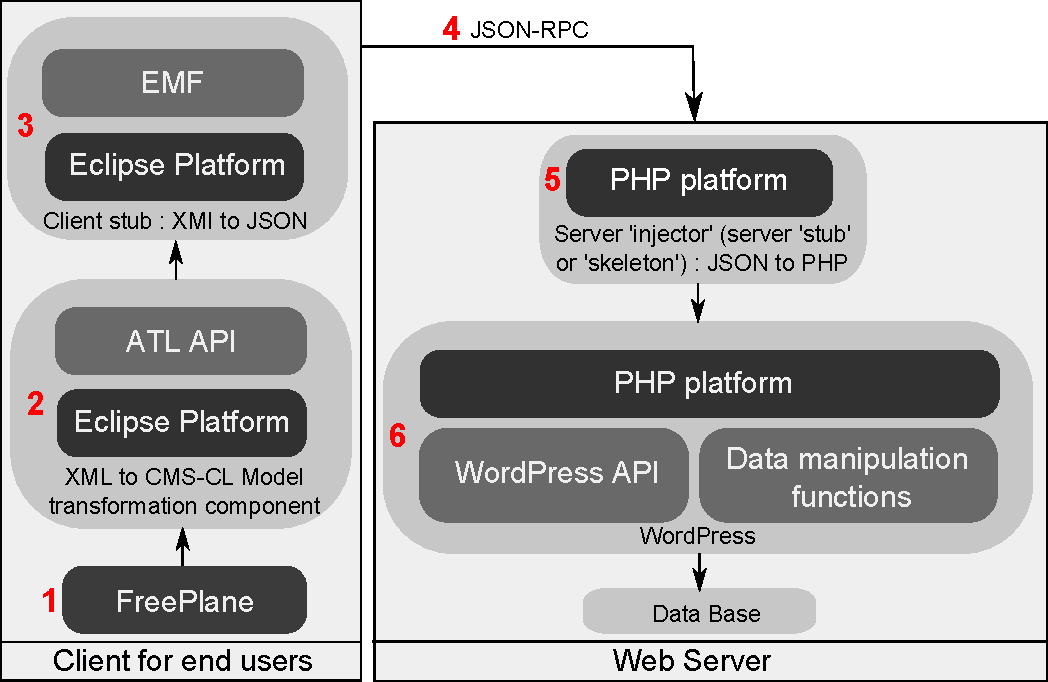
\includegraphics[width=0.85\textwidth]{../resources/pdf/final_ClientServer_numbered.pdf}
			\caption{Client-server complete process}
			\label{finalClientServer}
\end{figure}

	\subsection{Client part}	
		\vspace{0.15em}
		\noindent\textbf{Mind mapping (\textcolor{red}{1}).} To manipulate concepts with the mind mapping, the end-users use the Freeplane GUI and one of its output format which is the XML. With Freeplane, the users create a mind map (see section \ref{CMS-CL}, paragraph \ref{concreteSyntax}) of the different elements they want to manage for their web site.
%			\begin{figure}[!h]
%				\centering
%				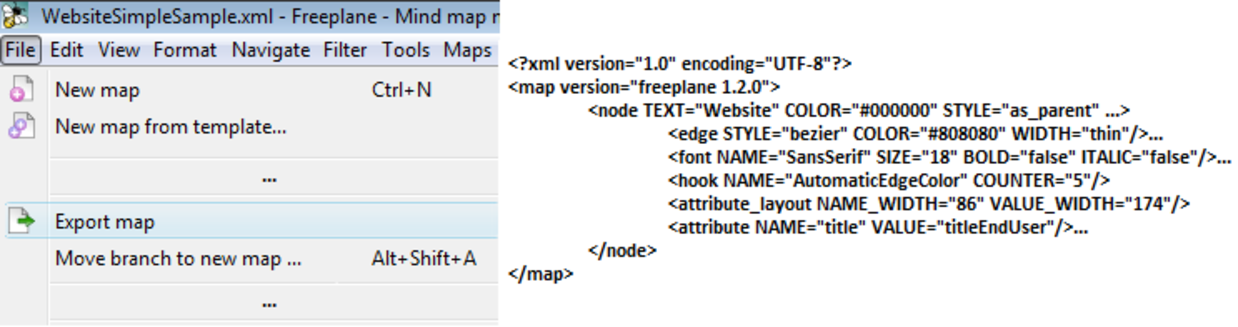
\includegraphics[width=\textwidth]{../resources/pdf/freePlaneUI_XML.pdf}
%				\caption{FreePlane : Export of the mind map and its xml output sample}
%				\label{freePlaneUI}
%			\end{figure}
			Then, via the export menu, they get a file representing this mind map, in an XML format\footnote{Extensbile Markup Language}\cite{xmlPresent}. There are other formats proposed (svg, mwiki, html, jpg, odt), but XML has some advantages that the other ones do not have : information structure is easily discerned by both humans and computers and it is application-independent.			
			
		\vspace{0.15em}
		\noindent\textbf{Transformation to CMS-CL model (\textcolor{red}{2}).} The XML representation must be now transformed in a CMS-CL model. For this, ATL\footnote{AtlanMod Transformation Language} is used : it is a model transformation language an Eclipse plugin. The output CMS-CL model is used by a third client component whose the description is done bellow.
		
		\vspace{0.15em}
		\noindent\textbf{Client 'stub' (\textcolor{red}{3}).} This component is called a 'stub' because it allows to have the same data format between the client and the server for the data interchange : the client parse (it is called 'marshalling') the data in JSON. So, the CMS-CL model is transformed to this common data interchange format by using the EMF\footnote{Eclipse Modeling Framework} \cite{emfPresent} on Eclipse.		
		The choosen format was JSON (see the listing\ref{jsonOutput} example) because it is specialized for data interchange, which is the case between the client and the server. It would be possible to have a direct transformation to this format (XML-to-JSON), but there are four reasons we choose to do this in two steps ('XML-to-CMS-CL' and 'CMS-CL-to-JSON') : \textit{Maintenability} (only the 'CMS-CL-to-JSON' transformation would be changed on a data interchange format modification),  \textit{Productivity} (if it is easier to maintain, it is also a gain of time), \textit{Readability} (with a one step process, we would have more complex metamodels, which is less readable), and \textit{Reusability} (each transformations could be usable by other components).
			\lstset{
  								caption=Web site elements in JSON, 
  								label=jsonOutput,
 								basicstyle=\scriptsize,
  								xleftmargin=.110\columnwidth , xrightmargin=.110\columnwidth
						}
			\begin{lstlisting}
{"website" : { "adminUser": { "idUser":"userOne", ... } }, ... }			
			\end{lstlisting}
	
	\subsection{Communication between Server and Client (\textcolor{red}{4})}
	The communication between the client and the server parts use the JSON-RPC\cite{jsonRpc} protocol : it uses the RPC protocol to call server methods, and the requests are in the JSON format.			
	\subsection{Server part}
		\textbf{Injector (server 'stub' or 'skeleton') (\textcolor{red}{5}).} This injector -also called the server 'stub' or 'skeleton'- consists to do the inverse of the 'stub' on the client side, i.e. to unparse the parameters (also called 'unmarshalling') and call its local WordPress functions with the parameters.
					
		\vspace{0.15em}
		\noindent\textbf{API and Data manipulations functions (\textcolor{red}{6}).} The functions called by the injector are divided in two types : those available in the WordPress API and those which are not remotely callable. But all of them send data to the data base, allowing a website update.	
	
	
\section{Validation}\label{validation}

The aim of this step was to validate the utility of the tool with end users. To do this, we created a simple use case\footnote{\scriptsize{Experimentation package: \url{https://drive.google.com/file/d/0B3kzMiMYv9r2ZXZ2c2VsTnA4WWM/edit?usp=sharing}}}, and retrieve users impressions via a questionnaire\footnote{\scriptsize{Questionnaire: \url{https://docs.google.com/forms/d/1MUKfjnyXrpKdfKZ5nnhYtUxyO11aOrRDad5KT2DM-3g/viewform}}}.

\subsection{Use case}
\vspace{0.15em}
\noindent\textbf{Mind-mapping process.}
During this step, the user must create mind-map, inject the elements in the WordPress CMS, and then observe the changes of the website. The provided mind-map for this test consisted of four components, as shown in Fig.\ref{mindMapUseCase}: Post, Page, User and Theme. But the user was always able to add a element choosed among these four types.

			\begin{figure}[!h]
				\centering
				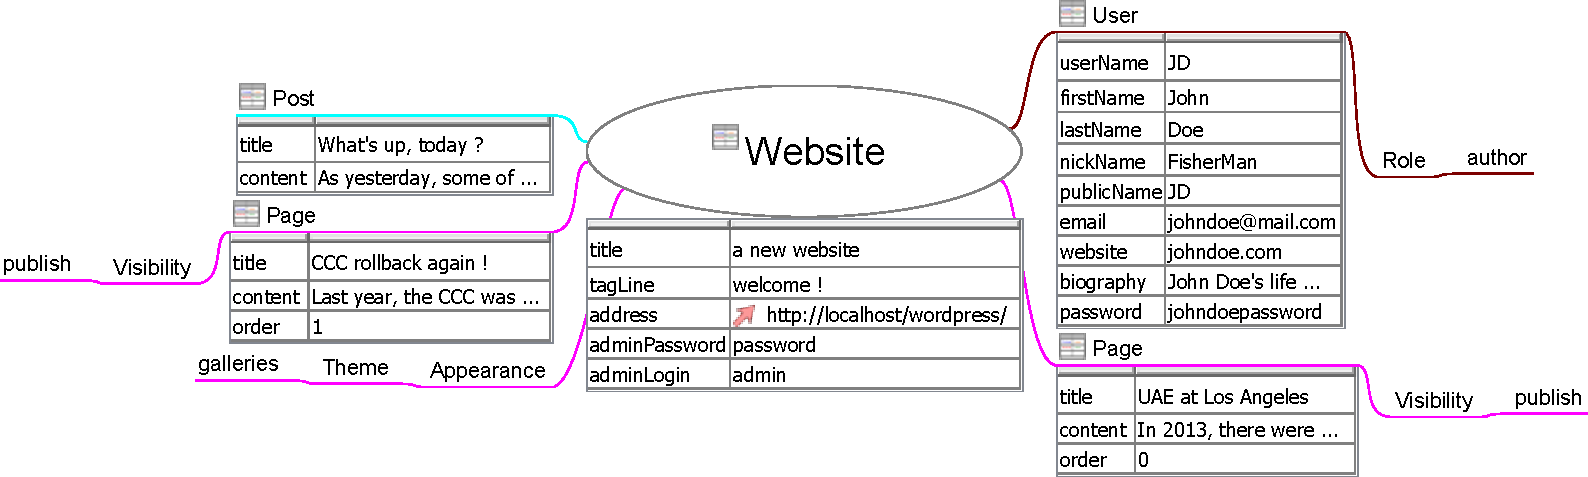
\includegraphics[width=\textwidth]{../resources/pdf/mindMapUseCase.pdf}
				\caption{Mind-map sample}
				\label{mindMapUseCase}
			\end{figure}

\vspace{0.15em}
\noindent\textbf{WordPress use.}
Users had to the same as in the previous step, but this time with WordPress, to be able to compare the two tools.

\vspace{0.15em}
\noindent\textbf{Comparison between WordPress and the mind-mapping process.}
Once both tools were used, users were able to give their opinion about the usefulness of a website configuration via a mind-mapping based DSL, by comparison to a tool such as WordPress.
	 
\subsection{Experimentation result}	 
\section{Textual representation and web designers}\label{webDesigners}
	\textbf{Approach.} 
	\begin{figure}[!h]
		\centering
		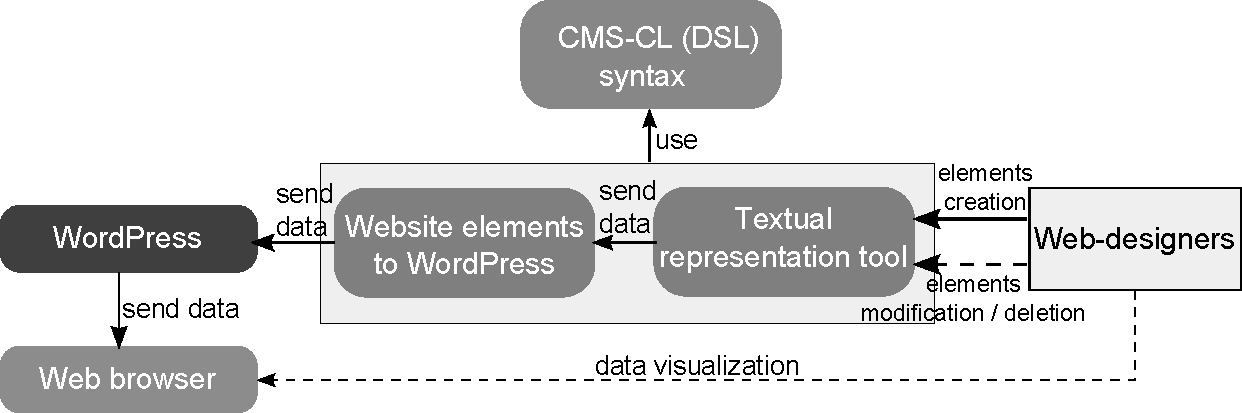
\includegraphics[width=\textwidth]{../resources/pdf/webDesignersSimplifiedPresentation.pdf}
		\caption{CMS-CL and textual representation tool}
		\label{CMS-CLIDEUse}
	\end{figure}
	Finally, the use of our defined DSL ('CMS-CL') with the textutal tool is the same than
	the one presented for end users (section \ref{approachOverview}), with just one modification about the component for the textual
	representation.		
	
	\vspace{0.15em}
	\noindent\textbf{CMS-CL Syntax.} The syntax for the web designers tool is quite the same than the end users one : there is an identic
	abstract syntax, but the concrete one is different because we choose a representation which is 
	textual\footnote{\scriptsize{'CMS-CL-to-XText' mapping:
	\url{https://raw.github.com/mallon/WordPress-MindMapping/master/Documentation/DetailedFigures/CMS-CL2XText.pdf}}}.
	
	A lot of tools allow textual representation, but we finally used XText~\cite{xtext}, because it is a framework specialized on
	the domain specific languages development : it has all the functionnalities than parser, linker, compiler or 
	interpreter have; but also because it is an Eclipse plugin and this IDE allows to have a reduce version of it 
	(called an Eclipse product~\cite{eclipseProduct}) with just some basic functionnalities and those we wanted (in our case : CMS-CL
	textual representation and compilation). Another reason is the active community behind it, and its	regular updates.	
	
	\vspace{0.15em}
	\noindent\textbf{Implementation} 	
	The technical part for the web designers changes just for the two first components on the client
	part, and uses the same stub than the end users technical part (see section \ref{techUse}). The server components does not change.
		
	\begin{figure}[!h]
		\centering
		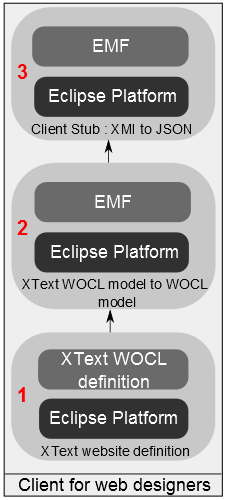
\includegraphics[width=0.90\textwidth]{../resources/pdf/final_WebDesignerClient_Server_numbered.pdf}
		\caption{Web designer (client) components}
		\label{wdCompos}
	\end{figure}		
		
	\vspace{0.15em}
	\noindent\textit{The first component (\textcolor{red}{1}) :} Enables to write a definition of the different elements that a web designers wants to 		add to a web site, using the XText grammar (those we have defined) respecting CMS-CL (the output being an XText CMS-CL model).
	
	\vspace{0.15em}
	\noindent\textit{The second component (\textcolor{red}{2}) :} Transforms the specific file format of the XText CMS-CL model to a file format (XMI) 		usable with the stub.
	
	\vspace{0.15em}
	\noindent\textbf{Use case.} With the Eclipse product, web designers can defined their website structure, as following List.\ref{textUse} shows, textually equivalent to the web site in section \ref{validation}.
	\lstset{
  								caption=Web site textual representation, 
  								label=textUse,
 								basicstyle=\scriptsize,
  								xleftmargin=.060\columnwidth , xrightmargin=.060\columnwidth
						}
	\begin{lstlisting}
<Website>
<adminUser elementContent={userOne}/>
<users listContent=[<User>
						<idUser content=userOne/>
						<userName content="admin"/>
						<password content="password"/>
						<userRole elementContent={administrator}/>
					</User>
]/>
					<Post>
						<idPost content=postOne/>
						<format elementCotnent={aside}/>
						<title content="'God Is An Astronaut' - Happy new year !"/>
						<content content="We would like to wish ..."/>
						<author elementContent={userOne}/>
					</Post>,
					<Post>...</Post>,
					<Post>...</Post>
...
</Website>											
\end{lstlisting}

%	\begin{figure}[!h]
%		\centering
%		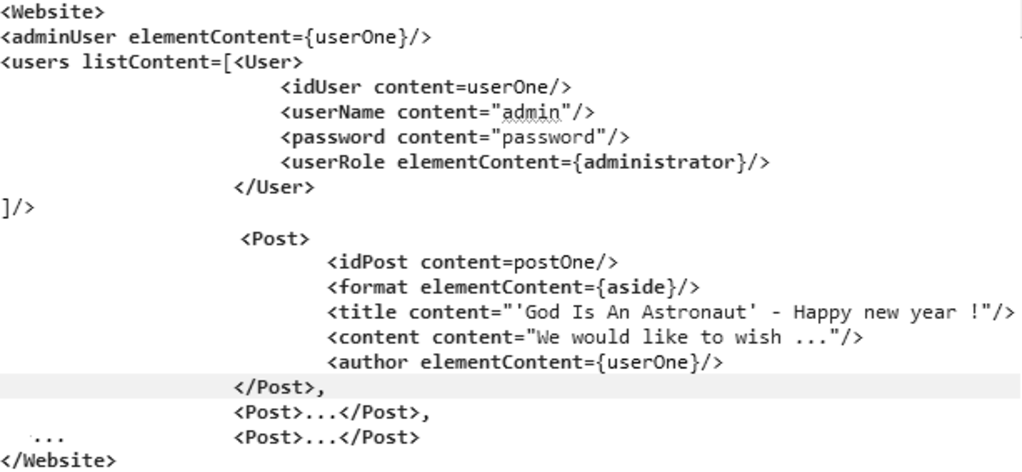
\includegraphics[width=0.90\textwidth]{../resources/pdf/webDesignersIde.pdf}
%		\caption{Web site textual representation}
%		\label{textUse}
%	\end{figure}
	
%	\textit{To inject data into WordPress}, web desginers have just to right-click on the configuration file.
%	\begin{figure}[!h]
%		\centering
%		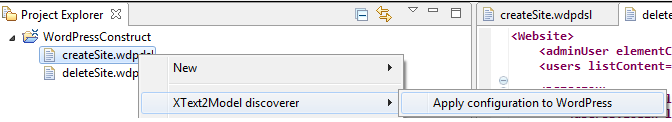
\includegraphics[width=0.90\textwidth]{../resources/pdf/webDesignersApplyConf.pdf}
%		\caption{Data injection}
%		\label{deleteElement}
%	\end{figure}	
	
	\vspace{0.15em}
	\noindent\textit{Modification:} It is the same as presented in section \ref{validation}.
	
	\vspace{0.15em}
	\noindent\textit{Deletion:} They have to use a \textit{'deletion'} tag, as in List.\ref{deleteElement}.
	\lstset{
  								caption=Deletion of a user with the 'Deletion' tag, 
  								label=deleteElement,
 								basicstyle=\scriptsize,
  								xleftmargin=.22\columnwidth , xrightmargin=.22\columnwidth
						}
	\begin{lstlisting}
<Deletion>
	<usersByLogin listContent=["nameUserOne"]/>
<\Deletion>
	\end{lstlisting}
	
%	\begin{figure}[!h]
%		\centering
%		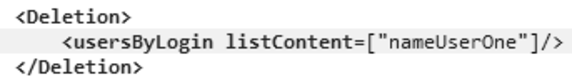
\includegraphics[width=0.5\textwidth]{../resources/pdf/deleteElement.pdf}
%		\caption{Deletion of a user with the 'Deletion' tag}
%		\label{deleteElement}
%	\end{figure}
	
\section{Related work}\label{relatedWorks}
The use of a DSL to simplify the web creation for end users was inspired by the
work of O.Diaz and G.Puente. In this paper, they present their own DSL - 'WSL' - for the creation of wiki via the mind mapping and the MediaWiki platform\cite{wikiScafolding}.

One other work\cite{conceptMod} focus on the data conceptual modelisation and communication to end users, using respectively two kinds of specific representation : an XML Document type Definition (DTD) and an XML Document Object Model (DOM).

Concerning a simpler (graphical) development support for more advanced end users (or developers), some other paper proposed a web interface, where the programming and the GUI creation processes are not separated\cite{livelyFabrik}. Their work is based on the Lively Kernel\cite{lively} of the Sun Labs.

Other works\cite{wsol,dslMashups} focusing more on functionalities, and more precisely on the proposed web services : they have made DSLs to improve the web services management, their compositions, and their creations.

Another tool \cite{dictator} enables to configure WordPress, but it is limited: indeed, it is technically only for the WordPress CMS (contrary to our tool, which could be easily applied to other CMS like Joomla or Drupal), and it uses a textual representation, which does not allow to have an equivalent quick and comprehensive overview of items added or changed.

Finally, a design tool using\cite{webRatio} a specific DSL was also proposed : with its specific DSL 'WebML', the tool allows designing complex Web and SOA\footnote{Service Oriented Architectures} applications, by providing visual design facilities and code generation. Because they used for the modeling step a representation which is less comprehensive for end users than a mind map and also because the textual representation make easier the web designer work, our tool and concepts could be integrate in it.
\section{Conclusion}
In this paper we have presented an approach allowing a simpler web site configuration for users. \textit{For this web site configuration}, we have used the \textit{WordPress CMS}, and \textit{our new DSL ('CMS-CL' : CMS Configuration Language)} to represent the WordPress configuration. Then, for the end users, we have used our DSL on top of the \textit{mind-mapping} to allow them to manipulate the different elements and easily configure the web site. About the web designers, we have created an IDE (using an Eclipse product and the XText plugin) using the DSL to textually defined the web site configuration.

As further work, it would be interesting to provide the possibility for end users to \textit{use our DSL in the same way, but collaboratively} : the DSL would be manuipulated online, and each authorized user could be able to manage web site elements, communicating with other users. In addition, \textit{this collaboration} between users \textit{could be apply on several sites}, i.e. a user could access to several online representations of different websites. The benefits given by this collaborative work platform would be the quality and speed improvement of the web sites creation. Another interesting thing, would be \textit{to create a more generalized DSL to use it with other CMS}.

\bibliographystyle{splncs}
\bibliography{Simplifying_access_to_the_creation_and_configuration_of_web_sites}

\end{document}